%\documentclass[preprint,tightenlines,showpacs,showkeys,floatfix,
%nofootinbib,superscriptaddress,fleqn]{revtex4} 
\documentclass[floatfix,nofootinbib,superscriptaddress,fleqn]{revtex4-2} 
%\documentclass[aps,epsfig,tightlines,fleqn]{revtex4}
\usepackage[utf]{kotex}
\usepackage[HWP]{dhucs-interword}
\usepackage[dvips]{color}
\usepackage{graphicx}
\usepackage{bm}
%\usepackage{fancyhdr}
%\usepackage{dcolumn}
\usepackage{defcolor}
\usepackage{amsmath}
\usepackage{amsfonts}
\usepackage{amssymb}
\usepackage{amscd}
\usepackage{amsthm}
\usepackage[utf8]{inputenc}
 \usepackage{setspace}
 \usepackage{tikz}
%\pagestyle{fancy}

\begin{document}

\title{\Large 2022년 1학기 물리학 I: Quiz 6}
\author{김현철\footnote{Office: 5S-436D (면담시간 매주
    화요일-16:00$\sim$20:00)}} 
\email{hchkim@inha.ac.kr}
\author{Lee Hui-Jae} 
\email{hjlee6674@inha.edu}
\affiliation{Hadron Theory Group, Department of Physics,
Inha University, Incheon 22212, Republic of Korea }
\date{Spring semester, 2022}


\vspace{1.cm}

\maketitle

\noindent {\bf 문제 1 [20pt]}
그림~\ref{fig:1}에서처럼 정지 상태에 있는 세 개의 블록을 가만히
놓았다. 이 세 블록은 $0.500\,\mathrm{m/s^2}$으로 가속한다. 블록 1은
질량이 $M$이고, 블록 2는 $2M$, 블록 3은 $2M$이다. 블록 2와 수평면
사이의 운동마찰계수를 구하여라.
\begin{figure}[ht]
  \centering
\includegraphics[scale=0.43]{Qfig6-1-20220321.png}  
  \caption{문제 1}
  \label{fig:1}
\end{figure}

\noindent {\bf 풀이:} 
우선 문제에 대한 자유물체 다이어그램을 그림~\ref{fig:2}와 같이
그리자. 

\begin{figure}[htp]
  \centering
  \begin{tikzpicture}
    \draw (-1.5,2.5) node {블록 1 :} ;
    \draw (0,-2.5) -- (0,2.5) ;
    \draw [blue,very thick,-latex] (0,0.1) -- (0,1.7) 
    node [left,black] {$T_1$};
    \draw [blue,very thick,-latex] (0,-0.1) -- (0,-1.2) 
    node [left,black] {$Mg$};
  \end{tikzpicture}
  \hspace{1.6cm}
  \begin{tikzpicture}
    \draw (-1.5,2.5) node {블록 2 :} ;
    \draw (-2.5,0) -- (2.5,0) ;
    \draw (0,-2.5) -- (0,2.5) ;
    \draw [red,very thick,-latex] (0,0.1) -- (0,2) 
    node [left,black] {$N$};

    \draw [blue,very thick,-latex] (-0.1,0) -- (-0.7,0) 
    node [above,black] {$T_1$};   
    \draw [blue,very thick,-latex] (-0.8,0) -- (-1.8,0) 
    node [below,black] {$f_k$};   

    \draw [blue,very thick,-latex] (0.1,0) -- (2,0) 
    node [above,black] {$T_2$};    
    \draw [red,very thick,-latex] (0,-0.1) -- (0,-2) 
    node [left,black] {$2Mg$};
  \end{tikzpicture}
  \begin{tikzpicture}
    \draw (-1.5,2.5) node {블록 3 :} ;
    \draw (0,-2.5) -- (0,2.5) ;
    \draw [blue,very thick,-latex] (0,0.1) -- (0,1.6) 
    node [left,black] {$T_2$};
    \draw [blue,very thick,-latex] (0,-0.1) -- (0,-2) 
    node [left,black] {$2Mg$};
  \end{tikzpicture}
  \caption{그림 2 : 블록 1,2,3 에 대한 자유물체 다이어그램}
  \label{fig:2}
\end{figure}
블록 1, 2, 3 에 운동 방향으로 작용하는 힘 $F$ 는 
다음과 같다. 
\begin{align}
  \begin{split}
    F &= (M+2M+2M)a=5Ma \\
    &=2Mg - Mg - f_k = Mg - f_k,
  \end{split}
\end{align}
$f_k$ 는 마찰력이다. 블록 2 에 작용하는 수직 항력을 $N$ 이라 하면,
\begin{align}
  f_k = \mu_kN.
\end{align}
블록 2에 수직 방향으로 작용하는 힘은 오직 중력 뿐 이므로, 
\begin{align}
  N = 2Mg = 2M\times(9.80\,\mathrm{m/s^2}).
\end{align}
따라서, 블록 1, 2, 3 에 작용하는 합력은 다음과 같다.
\begin{align}
  \begin{split}
    \sum F &= Mg - f_k = Mg - \mu_kN \\
    &= 5Ma= 5M \times (0.500\,\mathrm{m/s^2})
  \end{split}
\end{align}
운동 마찰 계수 $\mu_k$ 는 다음과 같다.
\begin{align}
  \begin{split}
    \mu_k &= \frac{Mg - 5M \times (0.500\,\mathrm{m/s^2})}{N} \\
    &= \frac{M\times((9.80\,\mathrm{m/s^2})-(2.50\,\mathrm{m/s^2}))}
    {2M\times(9.80\,\mathrm{m/s^2})}  \\
    &= 0.372
  \end{split}
\end{align}
운동 마찰 계수는 0.372 이다.


\vspace{2cm}

\noindent {\bf 문제 2 [10pt]} 프라이팬과 달걀 사이의 정지마찰계수는
$\mu_s=0.04$이다. 이 달걀이 프라이팬에서 미끄러지려면 프라이팬은
수평면으로부터 몇 도 기울어져야 하는가?  \\


\noindent {\bf 풀이:} 
프라이팬과 수평면이 이루는 각도를 $\theta$ 라고 하자. 달걀에 작용하는 힘을
프라이팬에 수직한 방향과 프라이팬에 평행한 방향으로 분해할 수 있다. 힘의 수직한
방향 성분을 $F_v$, 평행한 방향 성분을 $F_p$ 이라고 하면,
\begin{align}
F_v = mg\cos{\theta},\,\,\,F_p = mg\sin{\theta}  .
\end{align}
달걀은 힘 $F_v$ 로 프라이팬을 누르게 되고 프라이팬은 같은 크기로 달걀을 밀어내는데,
이 밀어내는 힘이 달걀에 작용하는 수직 항력이 된다.
이 달걀에 작용하는 수직 항력은 $F_v$ 의 반작용이므로 정지 마찰력 $f_s$ 는,
\begin{align}
  \begin{split}
    f_s &= \mu_s N = \mu_s F_v \\
    &= \mu_s mg\cos{\theta}.
  \end{split}
\end{align} 

\begin{figure}[htp]
  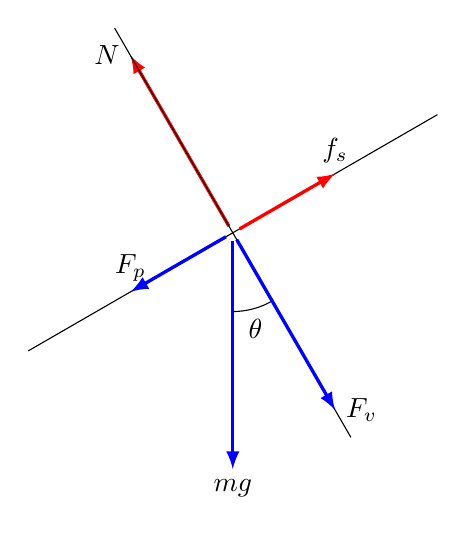
\begin{tikzpicture}
    \draw [rotate=30] (-3,0) -- (3,0) ;
    \draw [red,very thick,-latex,rotate=30] (0.1,0) -- (1.5,0) 
    node [above,black] {$f_s$};
    \draw [red,very thick,-latex,rotate=30] (0,0.1) -- (0,2.6) 
    node [left,black] {$N$};
    \draw [rotate=30] (0,-3) -- (0,3) ;
    \draw [blue,very thick,-latex] (0,-0.1) -- (0,-3) 
    node [below,black] {$mg$};
    \draw [blue,very thick,-latex,rotate=30] (0,-0.1) -- (0,-2.6) 
    node [right,black] {$F_v$};
    \draw [blue,very thick,-latex,rotate=300] (0,-0.1) -- (0,-1.5) 
    node [above,black] {$F_p$};
    \draw[black] (270:1) arc(270:300:1) (300:1) 
    node [below=10,left,black] {$\theta$};
  \end{tikzpicture} \caption{문제 2}
\end{figure}

달걀을 미끄러지게 하는 힘은 $F_p$ 이고 정지 마찰력 $f_s$ 는 이 힘과 반대 방향으로
작용한다. 달걀이 미끄러지기 위해서는 미끄러지게 하는 힘이 정지 마찰력 보다 커야한다. 즉,
\begin{align}
  F_p > f_s
\end{align}
이어야 한다. 따라서,
\begin{align}
  mg\sin{\theta}  > \mu_s mg\cos{\theta}
\end{align}
를 만족하는 가장 작은 $\theta$ 는 다음과 같이 구한다.
\begin{align}
  \tan{\theta} > \mu_s = 0.04
\end{align}
양변에 $\tan^{-1}$ 을 가해주면,
  \begin{align}
  \theta > \tan^{-1}{0.04} \approx 2.3^\circ
\end{align}
이므로 경사각이 $2.30^\circ$ 보다 커지면 달걀이 미끄러진다.
\vspace{2cm}

\noindent {\bf 문제 3 [20pt]}
짐을 실은 승강기의 총 질량이 
$1\,600\,\mathrm{kg}$이다. 초속도 2.00 m/s로 내려오던 승강기가 어느
순간부터 일정한 가속도로 감속하여 5.00 m 더 간 후
정지하였다. 정지하기까지 승강기를 연결한 줄의 장력은 얼마인가? (단,
중력가속도는 $9.80\,\mathrm{m/s^2}$이다.)   \\

\noindent {\bf 풀이 :}
\begin{figure}[htp]
  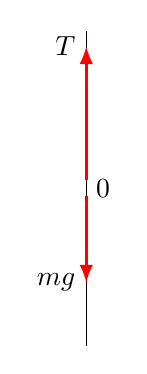
\begin{tikzpicture}
    \draw (0,-2.0) -- (0,2.0);
    
    \node[right] (X) at (0,0) {0};
    \draw [red,very thick,-latex] (0,0.1) -- (0,1.8) 
    node [left,black] {$T$};

    \draw [red,very thick,-latex] (0,-0.1) -- (0,-1.2) 
    node [left,black] {$mg$};
  \end{tikzpicture} \caption{Free body diagram}
\end{figure}
승강기는 어느 순간 부터 속력이 줄어드는 등가속도 운동을 하였으므로
 승강기에 가해진 가속도의 크기는 다음과 같다.
\begin{align}
  -2as = v^2-v_0^2,\,\,\, a = \frac{v_0^2-v^2}{2s}
\end{align}
승강기에 작용한 힘은 줄의 장력과 중력이다. 장력을 $T$ 라고 하면
 승강기에 작용한 합력은,
\begin{align}
  \sum F = ma = T-mg,\,\,\, T = m(a+g)
\end{align}
따라서 장력은 다음과 같다.
\begin{align}
  \begin{split}
    T  &= m(a+g)  \\ 
    &= (1\,600\,\mathrm{kg})\left(\frac{(2.00\,\mathrm{m/s})^2}
    {2(5.00\,\mathrm{m})}+9.80\,\mathrm{m/s^2}\right) \\
    &=1.63\times 10^4\,\mathrm{N}
  \end{split}
\end{align}
승강기에 작용한 줄의 장력은 $1.63\times 10^4\,\mathrm{N}$ 이다.




\vspace{2cm}

\noindent {\bf 문제 4 [40pt]} (\textbf{\color{red} 난이도 상})
질량이 각각 $m=16$ kg, $M=88$ kg인 두 블록이 
있다. 그림~\ref{fig:4}처럼 힘 $\vec{F}$를 가해 블록 $m$을 블록 $M$에
맞닿아 있도록 했다. 이 두 블록 사이의 정지마찰계수는
$\mu_s=0.38$이다. 블록 $M$이 놓여있는 수평면과 $M$ 사이에는 쓸림이
없다.  블록 $m$이 블록 $M$에서 미끄러져 내려오지 않도록 하는 데 필요한
최소힘 $\vec{F}$를 구하여라. 
\begin{figure}[ht]
  \centering
\includegraphics[scale=0.3]{Qfig6-4-20220321.png}  
  \caption{문제 4}
  \label{fig:4}
\end{figure}\\

\noindent {\bf 풀이 :} 

\begin{figure}[h]
  \begin{tikzpicture}
    \draw (-1.5,2.5) node {블록 $m$ :} ;
    \draw (-3,0) -- (3,0) node [above] {$+x$};
    \draw [red,very thick,-latex] (0.1,0) -- (2,0) 
    node [above,black] {$|\vec{F}|$};
    \draw [red,very thick,-latex] (-0.1,0) -- (-1.4,0) 
    node [above,black] {$N_m$};
    \draw (0,-2.5) -- (0,2.5) node [right] {$+y$};
    \draw [blue,very thick,-latex] (0,0.1) -- (0,1.5) 
    node [right,black] {$\mu_s N_m$};
    \draw [blue,very thick,-latex] (0,-0.1) -- (0,-1.5) 
    node [right,black] {$mg$};
  \end{tikzpicture} 
  \begin{tikzpicture}
    \draw (-1.5,2.5) node {블록 $M$ :} ;
    \draw (-3,0) -- (3,0) node [above] {$+x$};
    \draw [red,very thick,-latex] (0.1,0) -- (1.4,0) 
    node [above,black] {$N_m$};
    \draw (0,-2.5) -- (0,2.5) node [right] {$+y$};
    \draw [blue,very thick,-latex] (0,0.1) -- (0,2) 
    node [right,black] {$N_M$};
    \draw [blue,very thick,-latex] (0,-0.1) -- (0,-2) 
    node [right,black] {$Mg$};
  \end{tikzpicture} \caption{Free body diagram}
\end{figure}

두 물체의 가속도 $a$ 는 다음과 같다.
\begin{align}
  a = \frac{|\vec{F}|}{M+m}.
\end{align}
 블록 $m$ 이 블록 $M$ 에게 가하는 힘을 $N_m$ 이라고 하면,
 \begin{align}
   N_m = Ma = \frac{M}{M+m}|\vec{F}|
 \end{align} 
 블록 $M$ 은 이 힘의 반작용으로 같은 크기의 힘을 블록 $m$ 에게 가하고, 
 이 힘이 블록 $m$ 의 수직 항력이 된다. 블록 $m$ 이 정지해 있을 때 
 블록 $m$ 에 수직 방향으로 작용하는 힘의 합력은,
 \begin{align}
  \begin{split}
    F_y &= mg - \mu_s N_m = 0
  \end{split}
 \end{align}
 따라서 최소힘 $\vec{F}$ 의 크기는,
 \begin{align}
   \begin{split}
     N_m &= \frac{M}{M+m}|\vec{F}| =\frac{mg}{\mu_s},\,\,\,
     |\vec{F}| = \left(\frac{M+m}{M}\right)\left(\frac{mg}{\mu_s}\right)  \\
     |\vec{F}| &= \left(\frac{(88+16)\,\mathrm{kg}}{88\,\mathrm{kg}}\right)
     \left(\frac{(16\,\mathrm{kg})(9.80\,\mathrm{m/s^2})}{0.38}\right)  \\
     &= 4.9\times 10^2\,\mathrm{N}.
   \end{split}
 \end{align}
 블록 $m$ 이 미끄러지지 않기 위해 필요한 최소 힘은 $4.9\times 10^2\,\mathrm{N}$ 이다.
\end{document}